\providecommand\ExamFontPath{../../../字体/}
\documentclass[fontset=exam]{exam-zh}
\usepackage{longtable,booktabs,array,calc,multirow,fvextra}
\usepackage[normalem]{ulem}
\providecommand{\hl}[1]{#1}
\providecommand{\ul}[1]{\uline{#1}}
\DefineVerbatimEnvironment{verbatim}{Verbatim}{breaklines=true,fontsize=\small}
\providecommand{\tightlist}{\setlength{\itemsep}{0pt}\setlength{\parskip}{0pt}}
\newcommand{\pandocbounded}[1]{#1}
\setlength{\emergencystretch}{3em}
\setlength{\tabcolsep}{2pt}
\examsetup{page/size=a4paper}
\title{厦门大学 2011 级期末试卷}
\subject[4em]{力学}
\begin{document}
\maketitle
\fancyfoot[C]{第 \thepage 页（共 \pageref*{LastPage} 页）}
\pdfbookmark[1]{一． 判断题（每小题2分，共20分。正确的在相应序号后打“√”，错误的打“×”。要求将答案写在答题纸上）}{section1}

一． 判断题（每小题 2 分，共 20 分。正确的在相应序号后打``√''，错误的打``×''。要求将答案写在答题纸上）

\begin{enumerate}
\def\labelenumi{\arabic{enumi}.}
\item
  刚体对一系列平行轴的转动惯量中，对过质心那条轴的转动惯量最小。
\item
  当刚体作纯滚动时，作用在刚体上的静摩擦力总是与质心的运动方向相反。
\item
  作用在刚体上的外力的矢量和为零时，刚体的运动状态一定不变。
\item
  一波源产生的平面简谐横波一段时间后将振动传播至某质点，该质点初始振动方向取决于它离波源的位置。
\item
  高速运动电子的质量随其运动速率的增大而增大。
\item
  两同方向但不同频率的简谐振动合成后仍然为一简谐振动。
\item
  波速与质元的振动速度成正比。
\item
  流体微团的速度方向与通过该微团的流线的切线方向一致。
\item
  真空中的光速对任何惯性参考系都相同。
\end{enumerate}

10. 位移共振频率总是与振动系统的固有频率相同。

\pdfbookmark[1]{二．(16分) 如图，质量为m，长度为 l 的均匀细棒绕过O点的转轴自水平位置以零角速度自由下摆。求}{section4}

二．(16 分) 如图，质量为\(m\)，长度为 \(l\) 的均匀细棒绕过 O 点的转轴自水平位置以零角速度自由下摆。求

（1）细棒运动到与水平夹角为θ时的角加速度和角速度；\par\medskip{\centering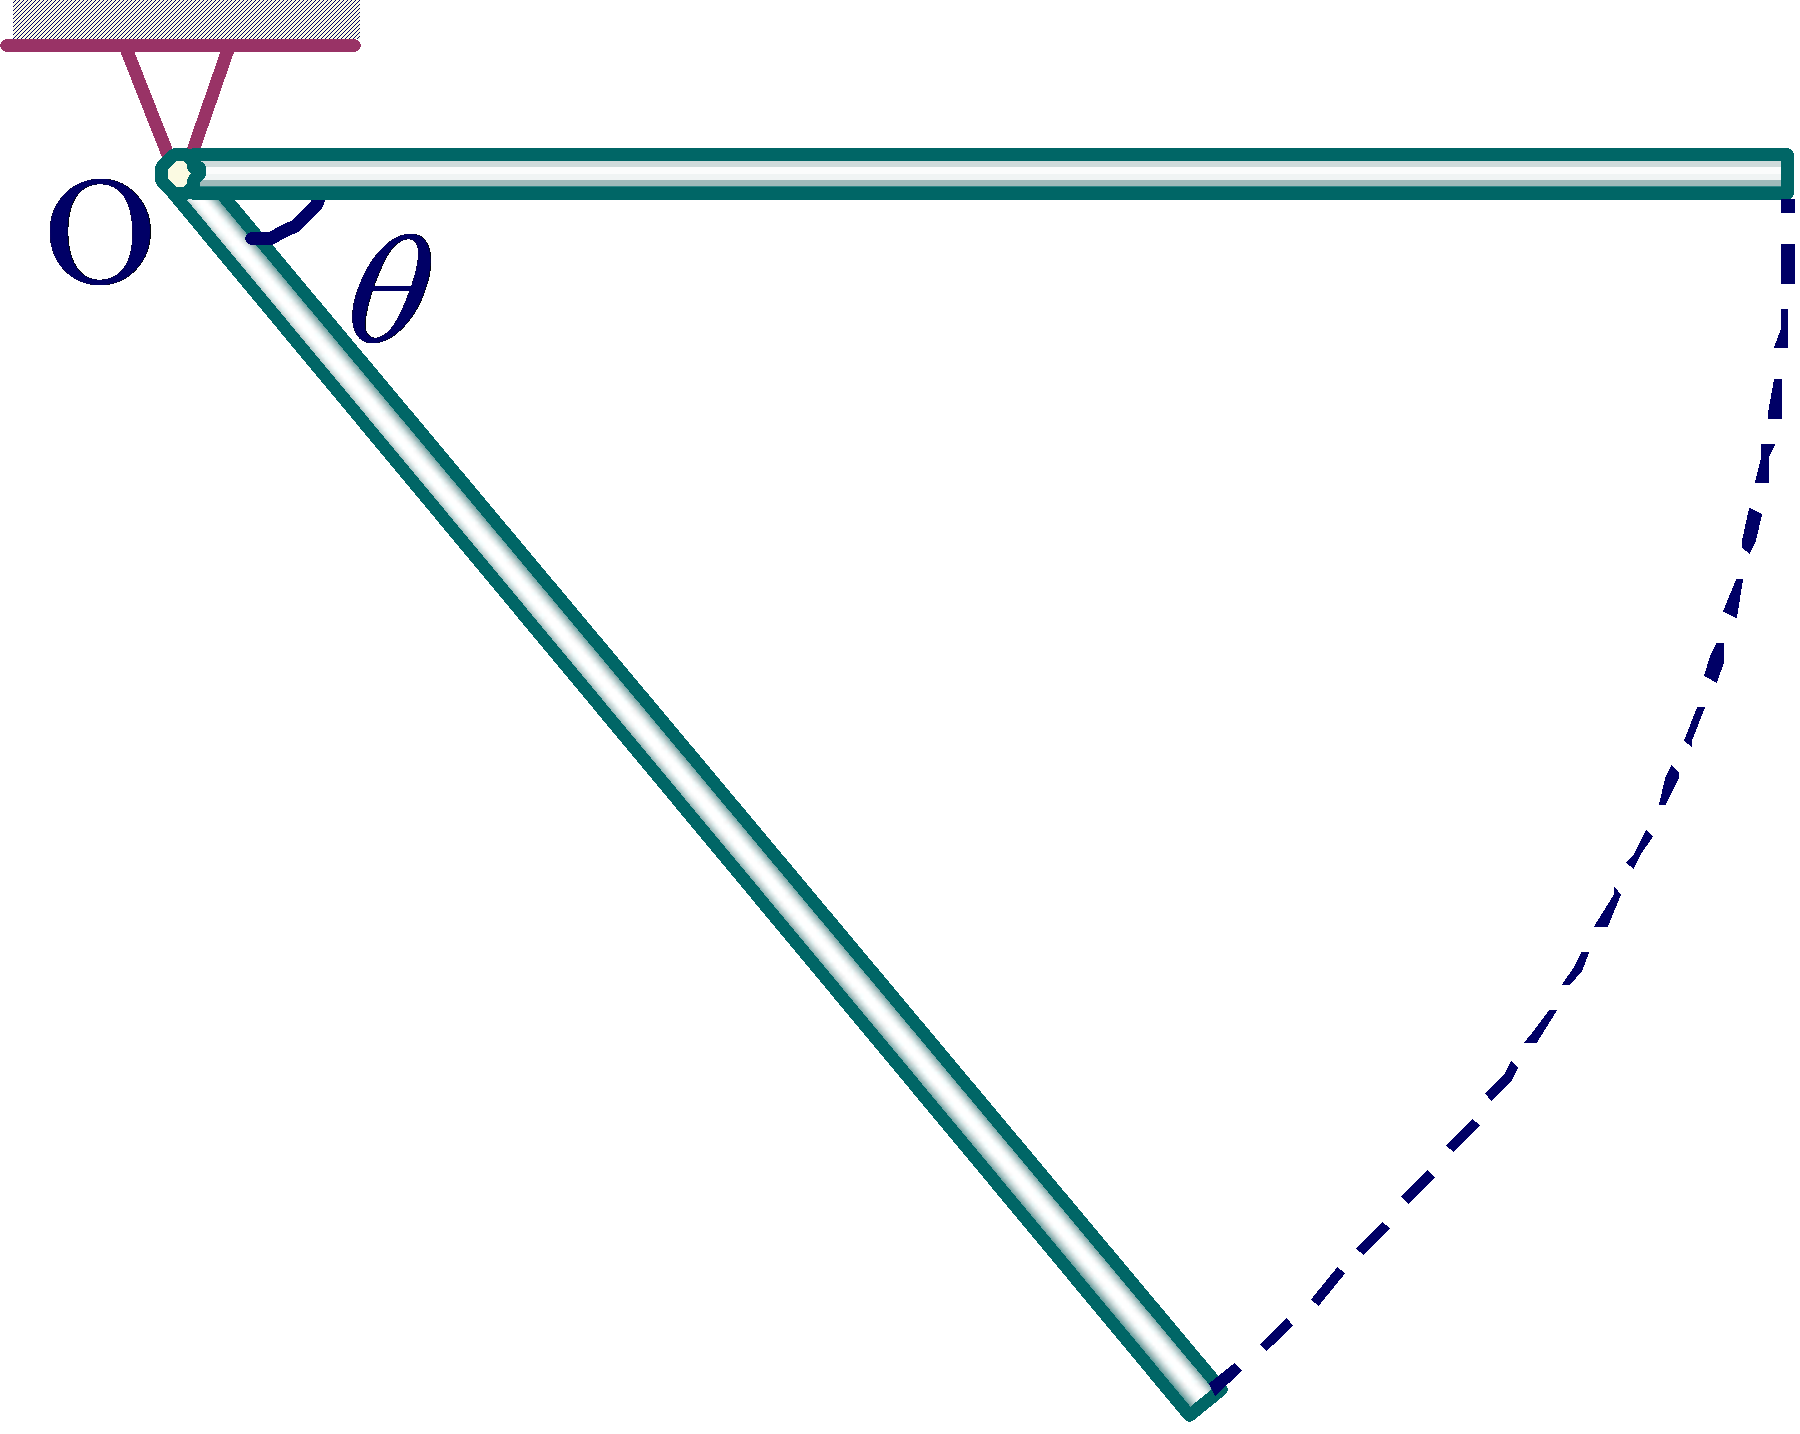
\includegraphics[width=5cm,height=4cm,keepaspectratio]{figures/image4.png}\par}\medskip

（2）此时细棒末端 A 的速度和加速度;

（3）求杆摆至竖直位置时，杆对支点的作用力。

\pdfbookmark[1]{三. (16分) 如图，水平桌面上的均质圆柱体A上绕着轻绳，绳子跨过一定滑轮B后与物体C相连。设A、B、C的质量均为为m}{section8}

三. (16 分) 如图，水平桌面上的均质圆柱体 A 上绕着轻绳，绳子跨过一定滑轮 B 后与物体 C 相连。设 A、B、C 的质量均为为 m，圆柱体和定滑轮的半径均为 R，现系统从静止开始运动。若圆柱体与各接触点、定滑轮与绳子间都无相对滑动，试求\par\medskip{\centering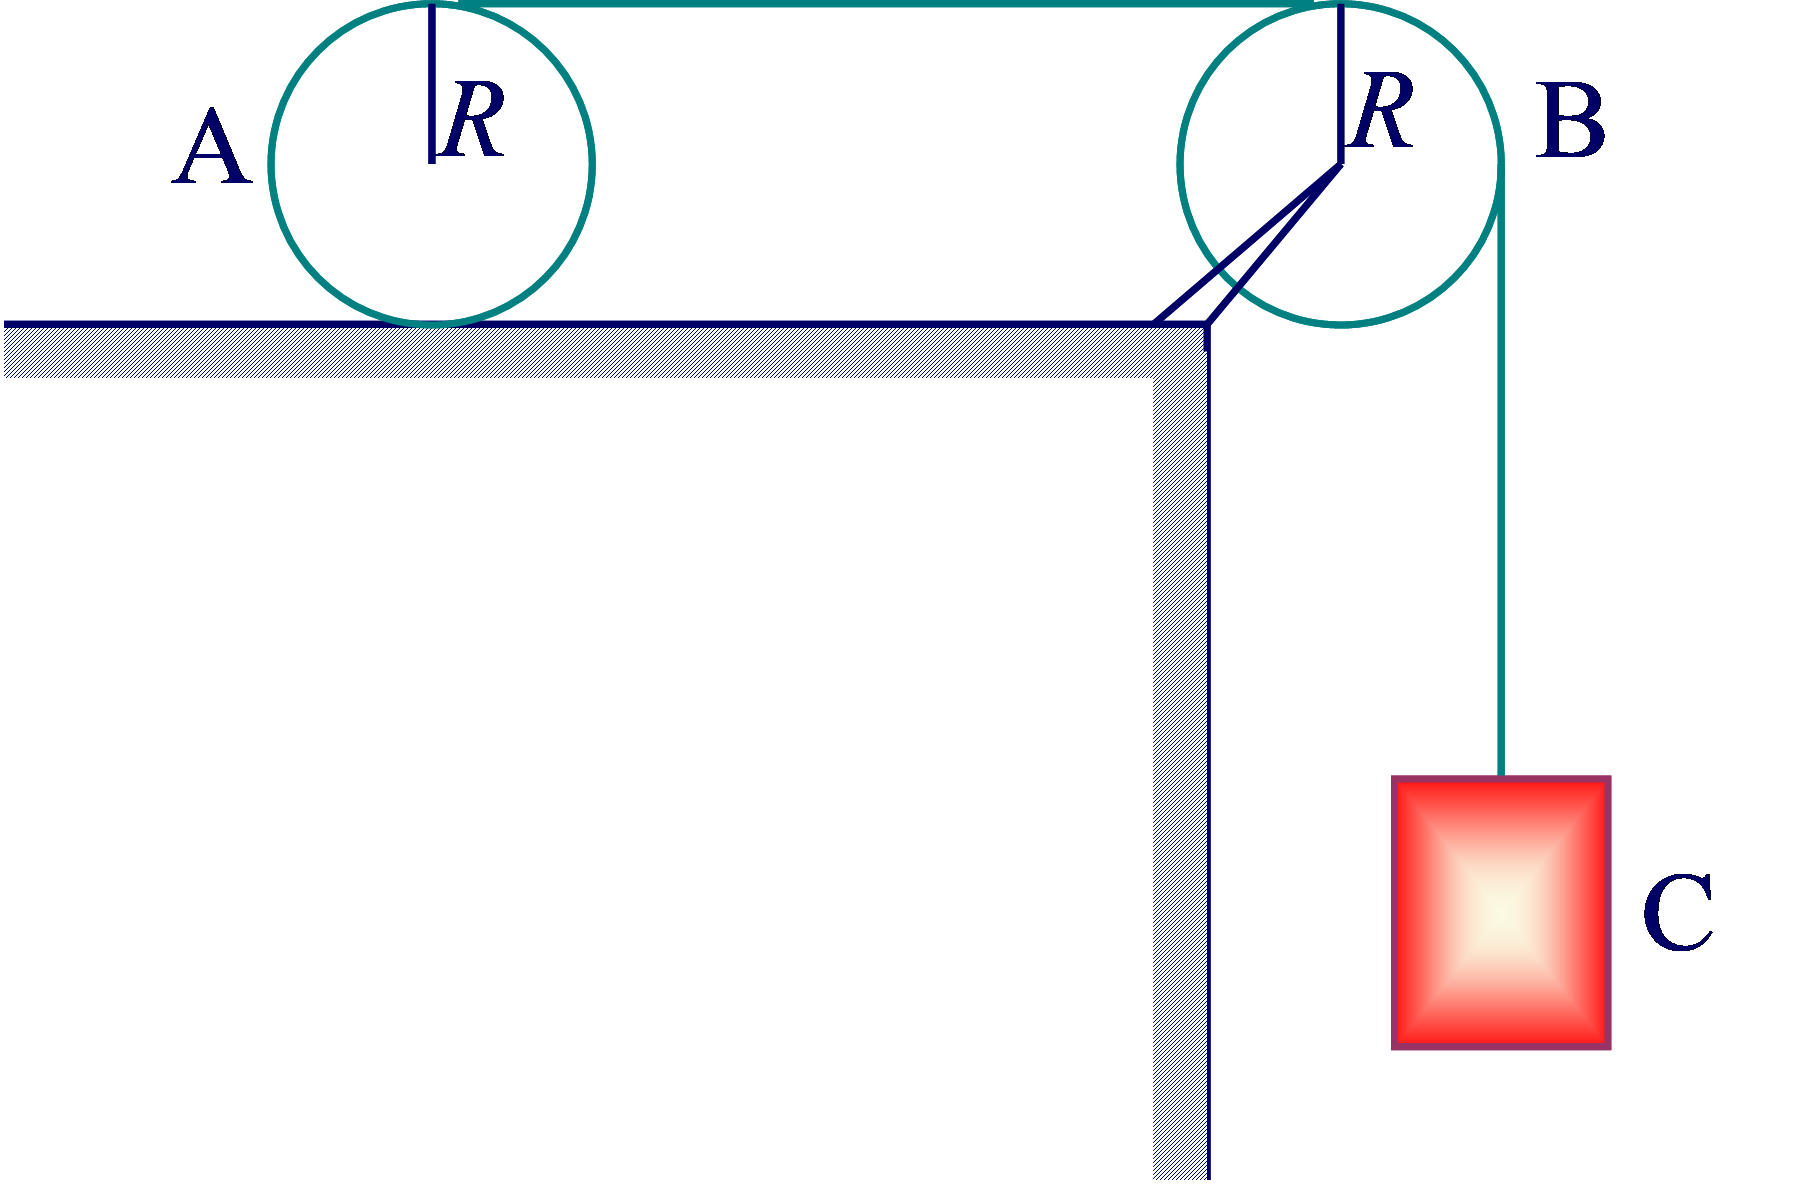
\includegraphics[width=5cm,height=4cm,keepaspectratio]{figures/image5.png}\par}\medskip

（1）圆柱体 A 与桌面间的摩擦力;

（2）物体 C 下落 h 后的速度和加速度大小。

\pdfbookmark[1]{四. (16分) 如图，水面上浮有一方形木块，在静止时水面以上高度为a , 水面以下高度为b . 木块密度为rho，水密}{section11}

四. (16 分) 如图，水面上浮有一方形木块，在静止时水面以上高度为 a , 水面以下高度为 b . 木块密度为\(\rho\)，水密度为\(\rho_{0}\)。现用外力将木块压入水中，使木快上表面与水面平齐. 设重力加速度为 g，不计水的阻力.

\par\medskip{\centering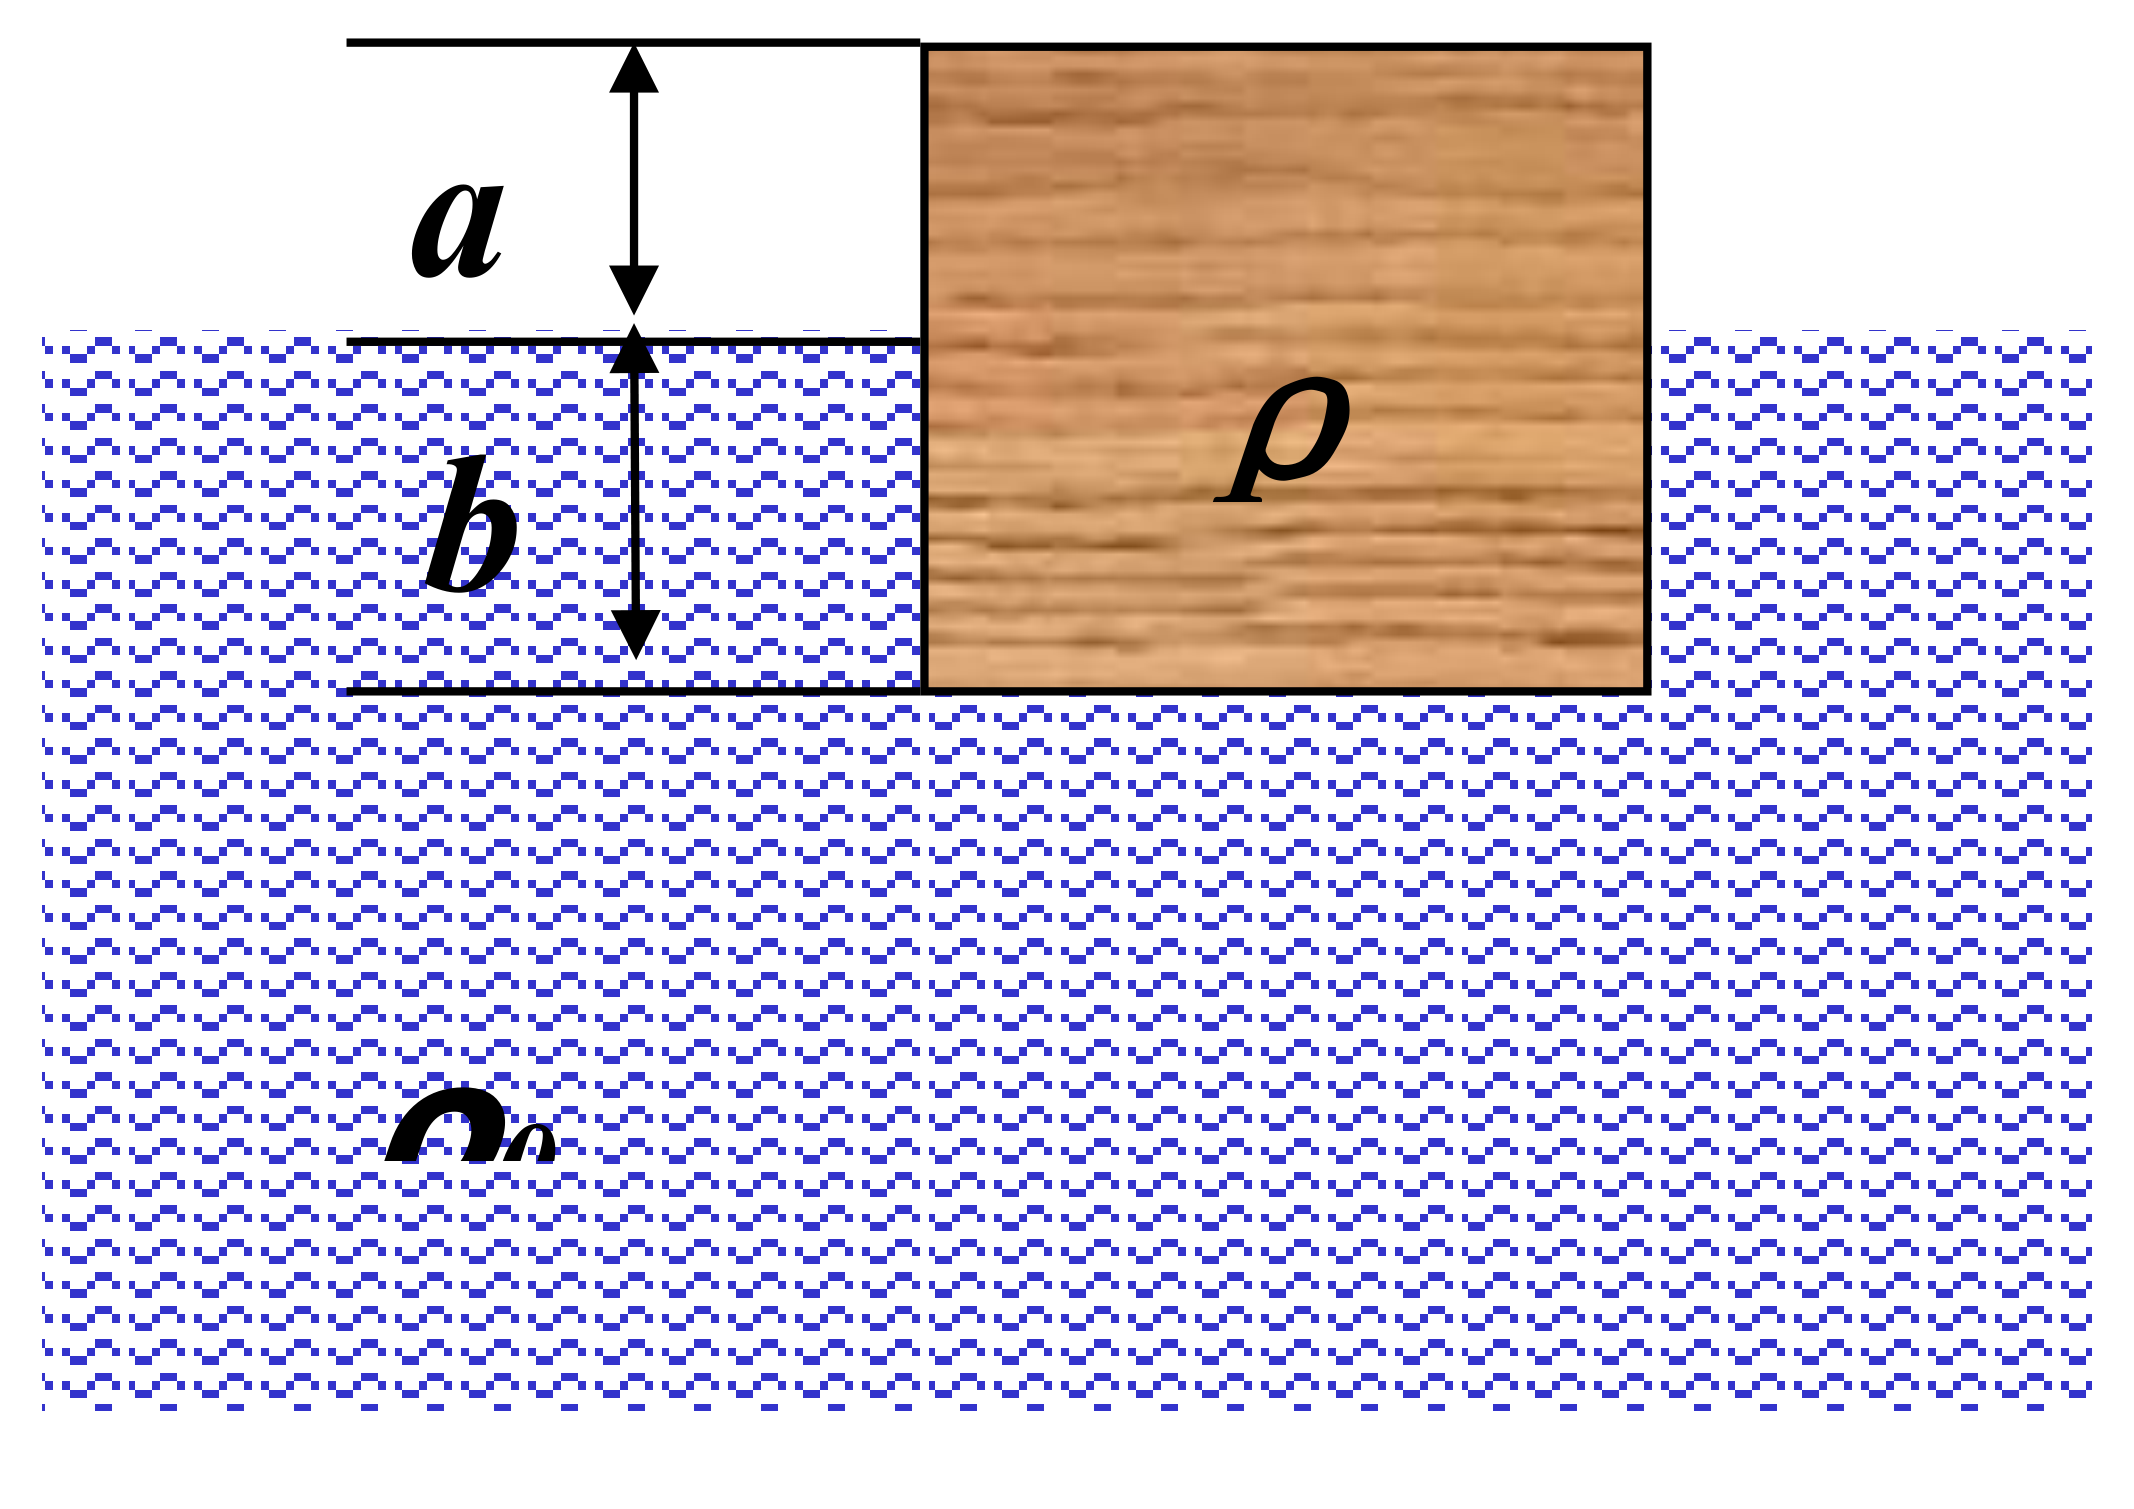
\includegraphics[width=5cm,height=4cm,keepaspectratio]{figures/wood4.png}\par}\medskip

（1）证明外力撤离后木块做简谐振动，并求出其振动周期;

（2）以水面所在高度为坐标原点，建立竖直向下的坐标系，并以木块第一次回到图示位置时为计时起点，写出该简谐振动的运动学方程。

\pdfbookmark[1]{五．(16分)原点处产生的一平面简谐波以波速u=4m/s沿x轴正方向传播，已知t=0时的波形图如图所示。若该波在x=L处}{section14}

五．(16 分)原点处产生的一平面简谐波以波速 u=4m/s 沿 x 轴正方向传播，已知 t=0 时的波形图如图所示。若该波在 x=L 处发生界面反射，且反射时无半波损失。试求:\par\medskip{\centering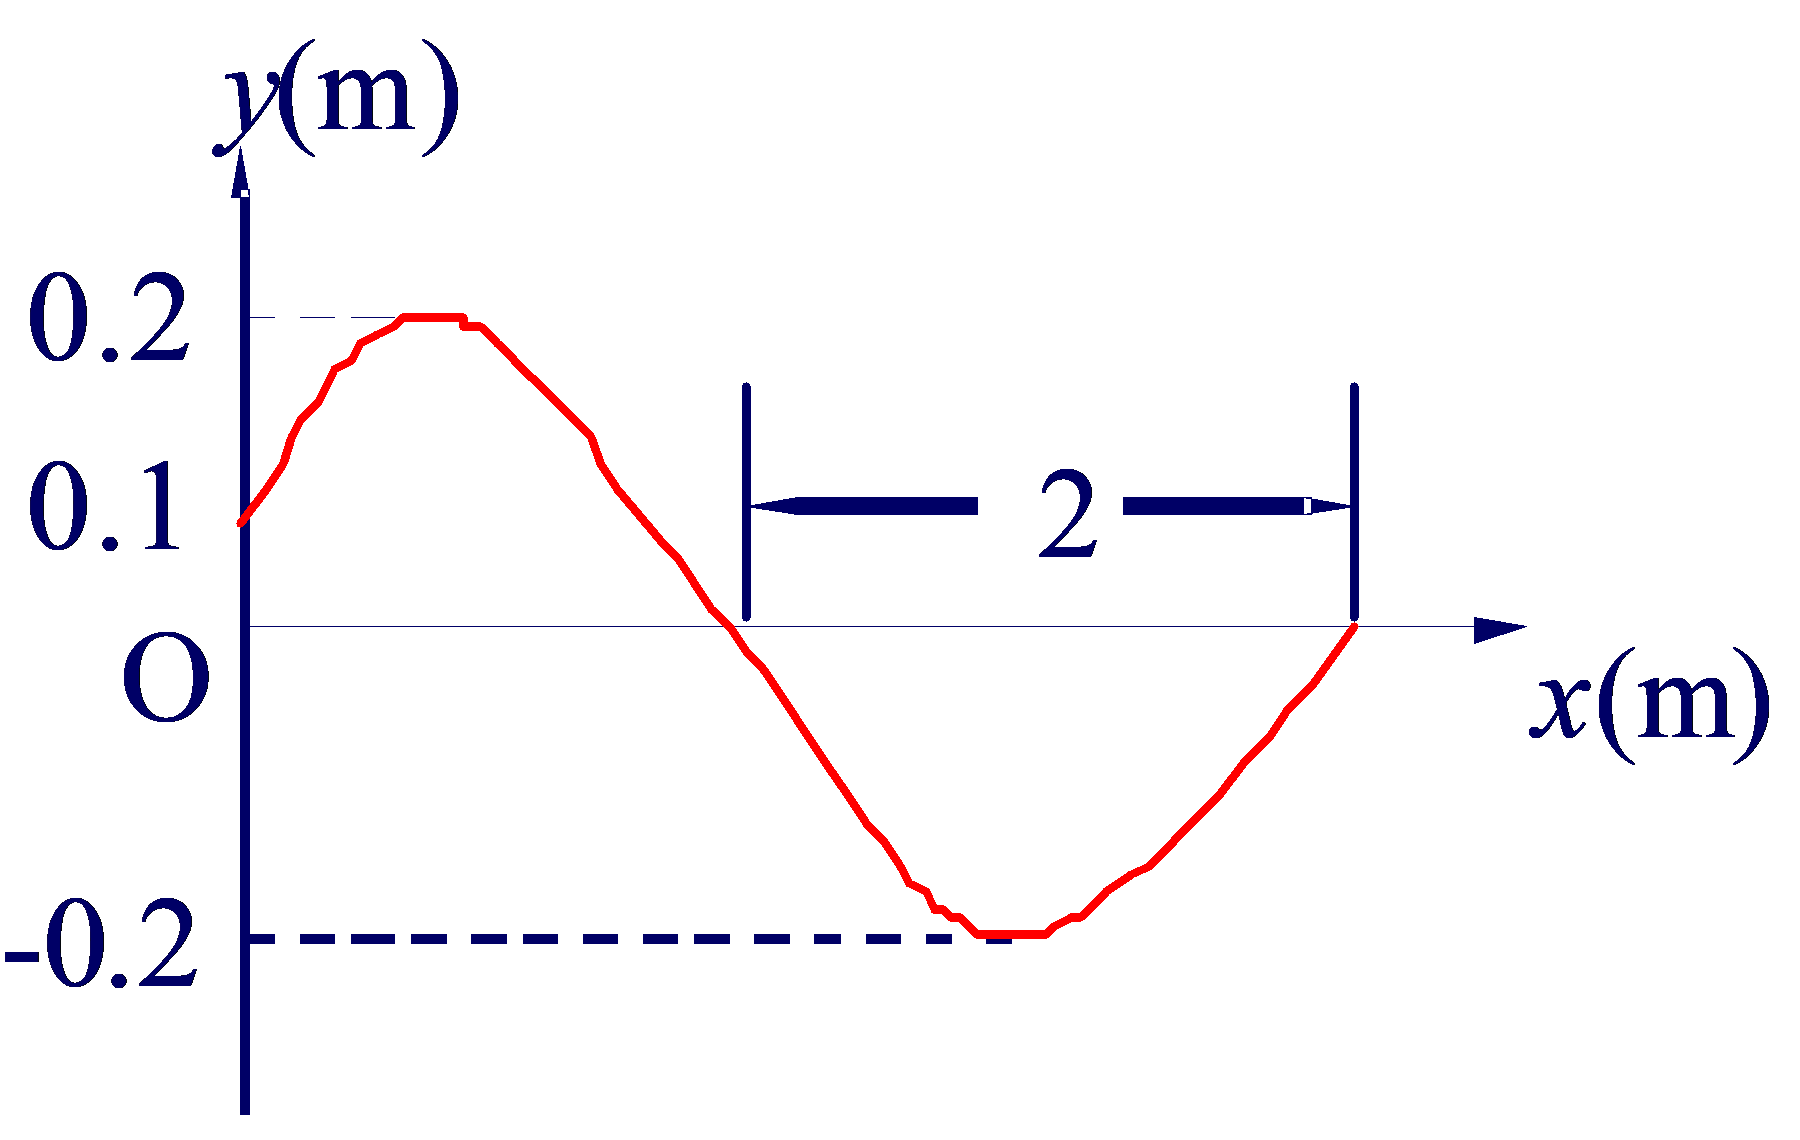
\includegraphics[width=5cm,height=4cm,keepaspectratio]{figures/image10.png}\par}\medskip

(1)原点处的振动方程

（2）该平面简谐波的波函数

(3)反射波的波函数（不考虑振幅衰减）

(4)若 L=10m 且波在反射时发生半波损失，请直接写出原点与反射点之间所有波节的位置坐标。

\pdfbookmark[1]{六. (16分) 一宇宙飞船A相对地面以0.8c的速度于正午时刻飞经地球，此时飞船和地球上的观测者都把自己的时钟拨到12}{section19}

六. (16 分) 一宇宙飞船 A 相对地面以 0.8c 的速度于正午时刻飞经地球，此时飞船和地球上的观测者都把自己的时钟拨到 12 点。宇宙飞船上的宇航员测得飞船的长度为 100 米。问：

（1）地面上的观测者测得的飞船 A 的长度为多少？

（2）按飞船上的时钟，宇航员于午后 12 点 30 分飞经一星际宇航站。该宇航站相对地球固定，其站台时间指示的是地球时间。问飞船到达此宇航站时，站台时钟显示的时间是多少？

（3）若有另一飞船 B 相对地面以 0.8c 的速度沿相反方向飞行，问 A 飞船上的观测者所测得的 B 飞船的速度大小。

\end{document}
